
\documentclass[tikz,convert={convertexe={magick.exe}}]{standalone}

\begin{document}
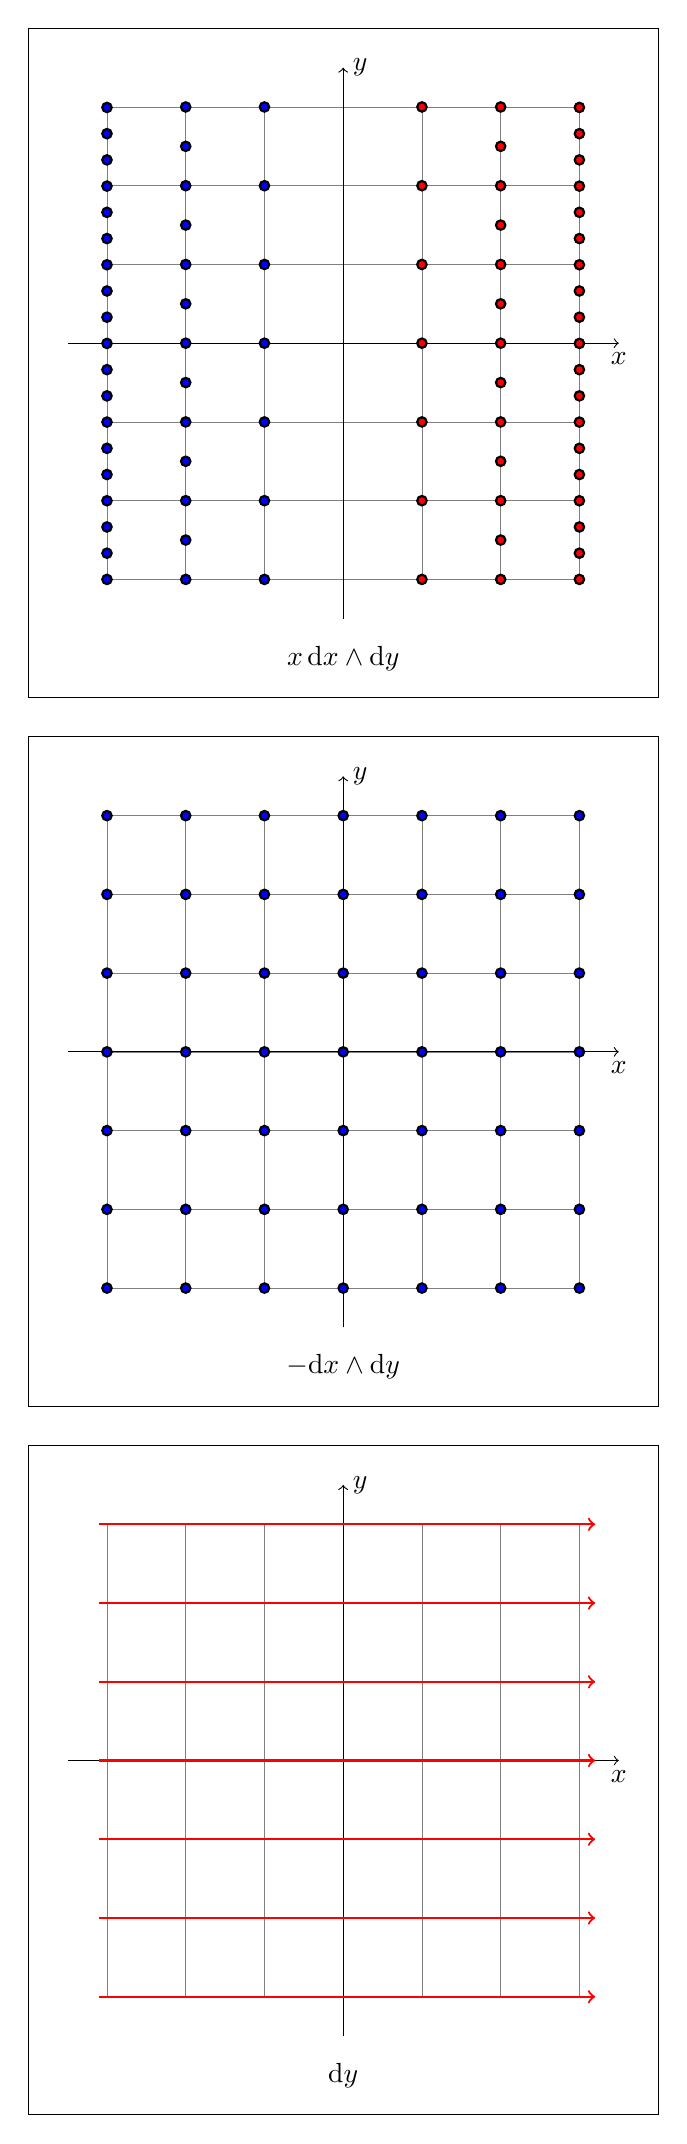
\begin{tikzpicture}

\tikzstyle atom=[circle, draw, inner sep=1.2pt, fill=red, thick]

\begin{scope}
\draw[style=help lines, very thin] (-3,-3) grid (3,3);

\draw[->] (-3.5,0)--(3.5,0) node[below] {$x$};
\draw[->] (0,-3.5)--(0,3.5) node[right] {$y$};

\draw (-4,-4.5) rectangle (4,4);
\node at (0,-4) {$x \, \mathrm{d}x \wedge \mathrm{d}y$};

\foreach \y in {-3,-2,...,3}
\node[atom] at (1,\y) {};
\foreach \y in {-3,-2.5,...,3}
\node[atom] at (2,\y) {};
\foreach \y in {-3,-2.667,...,3}
\node[atom] at (3,\y) {};


\foreach \y in {-3,-2,...,3}
\node[atom, fill=blue] at (-1,\y) {};
\foreach \y in {-3,-2.5,...,3}
\node[atom, fill=blue] at (-2,\y) {};
\foreach \y in {-3,-2.667,...,3}
\node[atom, fill=blue] at (-3,\y) {};
\end{scope}

\begin{scope}[yshift=-9cm]
\draw[style=help lines, very thin] (-3,-3) grid (3,3);

\draw[->] (-3.5,0)--(3.5,0) node[below] {$x$};
\draw[->] (0,-3.5)--(0,3.5) node[right] {$y$};

\draw (-4,-4.5) rectangle (4,4);
\node at (0,-4) {$- \mathrm{d}x \wedge \mathrm{d}y$};

\foreach \x in {-3,-2,...,3}
\foreach \y in {-3,-2,...,3}
\node[atom, fill=blue] at (\x,\y) {};
\end{scope}

\begin{scope}[yshift=-18cm]

\foreach \x in {-3,-2,...,3}
\draw[style=help lines, very thin] (\x,-3) -- (\x,3);

\draw[->] (-3.5,0)--(3.5,0) node[below] {$x$};
\draw[->] (0,-3.5)--(0,3.5) node[right] {$y$};

\draw (-4,-4.5) rectangle (4,4);
\node at (0,-4) {$\mathrm{d}y$};

\foreach \y in {-3,-2,...,3}
\draw[red, thick, ->] (-3.1,\y) -- (3.2,\y);
\end{scope}

\end{tikzpicture}
\end{document}